\documentclass[12pt]{exam}         %% What type of document you're writing.

%%%%% Preamble

%% Packages to use

\usepackage{amsmath,amsfonts,amssymb}   %% AMS mathematics macros
\usepackage{lettrine}
\usepackage{graphicx}
\usepackage[export]{adjustbox}
\usepackage{tikz}
\usepackage{polyglossia}
\usepackage{xcolor}
\usepackage{longtable}
\usepackage{fontawesome}
\usepackage{xparse}
\usepackage{hyperref}

\hypersetup{
    colorlinks=true,
    linkcolor=blue,
    filecolor=magenta,
    citecolor=blue,
    urlcolor=purple,
}

\setdefaultlanguage{english}
\setmainfont[Language=English]{DejaVu Sans}
%\setmainfont[Language=English]{Gentium Book Basic}
% math font sizes
\DeclareMathSizes{12}{16}{14}{12}
% see https://tex.stackexchange.com/questions/75284/how-do-i-write-a-recurring-decimal-in-latex
\ExplSyntaxOn
%% Dots on the first and last digit
\NewDocumentCommand{\periodfl}{m}
 {
  \repdec_initial_final_dots:n { #1 }
 }

\seq_new:N \l__repdec_digits_seq
\tl_new:N \l__repdec_first_tl
\tl_new:N \l__repdec_last_tl

\cs_new_protected:Npn \repdec_initial_final_dots:n #1
 {
  \seq_set_split:Nnn \l__repdec_digits_seq {} { #1 }
  \seq_pop_left:NN \l__repdec_digits_seq \l__repdec_first_tl
  \seq_pop_right:NN \l__repdec_digits_seq \l__repdec_last_tl
  \quark_if_no_value:VF \l__repdec_first_tl { \dot{\l__repdec_first_tl} }
  \seq_use:Nnnn \l__repdec_digits_seq {}{}{}
  \quark_if_no_value:VF \l__repdec_last_tl { \dot{\l__repdec_last_tl} }
 }
\cs_generate_variant:Nn \quark_if_no_value:nF { V }
\ExplSyntaxOff

% total counter
\usepackage{totcount}
% total counter

%% Title Information.

\title{The Term-end Math Exam\footnote{The exam is for Rujuta Mhaswade, age 12, at the Free Learner's School, but anyone can enjoy it. The exam is free for anyone to take!}}
\author{Kedar Mhaswade\footnote{Student and Teacher at the Free Learner's School.}}
\date{May 2021}

\setlength{\parindent}{0pt}% Remove paragraph indent
\usepackage[skip=\medskipamount]{parskip} % each paragraph has whitespace

\begin{document}

\maketitle

\lettrine[lines=3]{A}{LRIGHT}! The so-called term-end exam is here. Since we do everything for fun, we take exams lightly as well!  This text consists of problems that should be attempted for fun, but as part of an exam, so that you get used to the excitement, anxiety associated with it. After all, right now, exams is how the world tries to evaluate you. So, it helps you to get that experience. And you know, sometimes stress brings out our best response to it! 
The exam is based on what we have learned so far, however, that is just to be used as a guidance. Find out what \emph{kind} of problems are challenging and then perhaps work on the fundamentals to strengthen your understanding.


Some things to keep in mind:
\begin{enumerate}
\item It may be a good idea to print this out on both sides of a paper and attempt the answers with a pen or pencil on a separate paper. You may choose to use Google Docs instead as well. 
\item A quiz may contain errors. If a question is unclear, be sure to get it clarified.
\item It is a quiz of sorts. The time is not really limited, but you should plan on focusing for about an hour each time you take the quiz. Try to attempt as many problems as you can in a couple of days. Remember, it is a marathon, not a 100-meter dash.
\item Give each problem enough thought and time and then present your solutions.
\item Have fun. Hopefully you will struggle to get through the problems. Perhaps you will make silly mistakes. Don't worry, it is all part of the game. You will get better only if you have fun doing it. Note that some problems may be difficult and you may be stuck. \emph{Being stuck is okay}. Note that some of these problems have been (or still are) difficult for me too.
\item For the sake of examination, the correct solution (however you find it) to every problem carries points indicated in a pair of parentheses. Giving points to solutions is, of course, pointless, but let's just do it for the sake of it and hope that we have some fun along the way. 
\item You are allowed to use a calculator. But try to do calculations in your head or on paper. It helps.
\item Be honest.
\end{enumerate}

\begin{center} {\Large \textbf{Good Luck}!} \end{center}

\medskip
\par\noindent\rule{\textwidth}{0.4pt}


\newtotcounter{totpoints}
{\Large Points: \total{totpoints}}

\newcommand\Prob[2]{
    \leavevmode\par
    \stepcounter{question}
    \noindent
    \addtocounter{totpoints}{#2}
    \textbf{Problem \thequestion \space (#2 points)} -- #1 \par
   }

\newcommand\Ans[2][]{%
    \leavevmode\par\noindent
    {\leftskip37pt
    A --- \textbf{#1}#2\par}
   }

\par

\Prob{
See Figure \ref{fig: num-col}. 
\begin{figure}[h!]
    \centering
    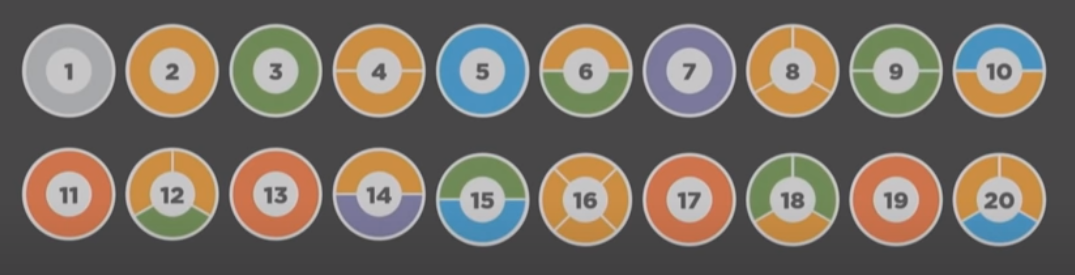
\includegraphics[width=1.0\linewidth]{numbers-and-colors.png}
    \caption{The First 20 Numbers}
    \label{fig: num-col}
\end{figure}

\begin{enumerate}
    \item How will you draw and color numbers $21$, $22$, and $23$?
    \item Which is the first number after $1$ that will have a gray?
\end{enumerate}
}{2}

\Prob{
\begin{figure}[htbp!]
    \centering
    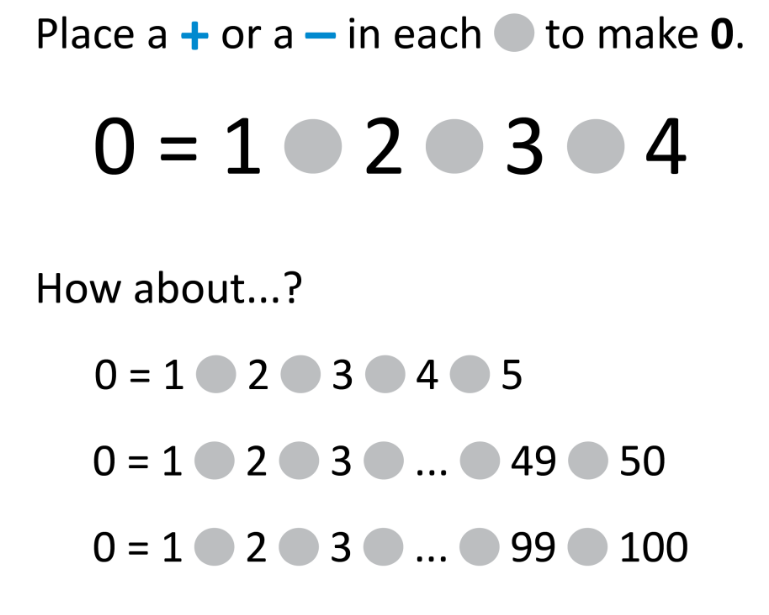
\includegraphics[width=0.6\linewidth, frame]{minus-plus.png}
    \caption{Minus Plus}
    \label{fig: minus-plus}
\end{figure}
    Solve the problem in Figure \ref{fig: minus-plus}. This is one of the things that mathematicians do: Generalization, wherein after solving a few concrete problems, they try to find a pattern. To achieve such a goal, they have to play with things at hand, just like what you are doing right now!
}{10}

\newpage

\Prob{
    What is the difference between $(a^b)^{c}$ and $(a)^{b^c}$? Give an example or two.
}{2}

\Prob{
    Find the values of $A$, $B$, and $C$ from the following sum:

    \begin{center}
    \begin{tabular}{cccc}
        & $A$ & $B$ & $C$ \\
      + & $A$ & $B$ & $C$ \\
      + & $A$ & $B$ & $C$ \\
      \hline
        & $B$ & $B$ & $B$ \\
    \end{tabular}
    \end{center}
}{3}

\Prob{
    One of my favorite theorems is the \emph{Fundamental Theorem of Arithmetic} (FTA) which simply states that every integer, $N$, can be expressed as a product of prime numbers (each of these is a \emph{prime factor} of $N$) in a unique way. Explain what one means by ``reducing a fraction to its lowest terms''. How can one use the FTA to reduce a fraction to its lowest terms? Reduce this fraction to its lowest terms: 
    $$
        \dfrac{\, 13\, }{\frac{39}{2}}
    $$

    And Oh, by the way, is the above fraction same as 
    $$
        \dfrac{\, \frac{13}{39}\, }{\, 2\, } 
    $$
    ?

    I agree, this may be seen as a problem with the way we write in mathematics -- the so called ``mathematical notation'' -- but you know, we have got to become familiar with the alphabet if we need to read anything.
}{4}

\Prob{
    \emph{Unit fractions} are, as you might have guessed, fractions with the numerator 1 and the denominator a positive integer. Thus, $\dfrac{1}{7}$, $\dfrac{1}{12}$ are unit fractions, whereas $\dfrac{3}{4}$ and $\dfrac{2}{7}$ are not.

    It is said that we can express \emph{any} non unit fraction as a \textbf{sum of unit fractions} whose denominators are different. For example, 

    $\dfrac{5}{8} = \dfrac{1}{4} + \dfrac{1}{8}$,

    or

    $\dfrac{2}{3} = \dfrac{1}{2} + \dfrac{1}{6}$

    Express the following fractions as a sum of unit fractions with different denominators: 
    \begin{enumerate}
        \item $\dfrac{3}{8}$
        \item $\dfrac{3}{7}$
        \item $\dfrac{7}{11}$
    \end{enumerate}

    Hint: The first unit fraction is clearly $\dfrac{1}{2}$. Perhaps you can look at your fraction and $\dfrac{1}{2}$ and you might see something and an algorithm will emerge?

}{15}

\Prob{
\begin{figure}[h!]
    \centering
    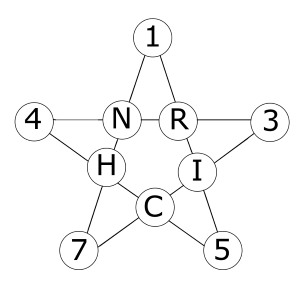
\includegraphics[width=0.3\linewidth, frame]{nrich-star.png}
    \caption{Star Sum}
    \label{fig: nrich-star}
\end{figure}

In the star shown in Figure \ref{fig: nrich-star} the sum of the four numbers in any ``line" is the same for each of the five ``lines".  The five missing numbers are $9$, $10$, $11$, $12$, $13$.

Which number is represented by R?

}{5}

\Prob{
    Here is a curious fact about numbers $3$ and $2$. If I add them, I get $5$, but I also get $5$ if I subtract their squares:
    $$
        3 + 2 = 5
    $$
    $$
        3^2 - 2^2 = 9 - 4 = 5
    $$

    Do you think this happens \emph{only} for $3$ and $2$, or do you suppose their are other numbers for which this might work?
}{10}

\Prob{
    If $m$ and $n$ are integers (that is, $m, n \in \mathbb{N}$) and $m + n$ is even, then $m-n$ is even. 
    
    Prove or disprove the above statement.
}{5}

\Prob{
    I am thinking of an integer $n$ that is divisible by $11$. $n$ also leaves a remainder $1$ when divided by $3$ and a remainder $3$ when divided by $5$.

    Find $n$.

    Is $n$ unique, or are there more numbers that behave this way?
}{10}

\Prob{
    Express the decimal fraction $0.461538461538\dots$ -- which can be denoted as $0.\periodfl{461538}$ -- as a common fraction.
}{2}

\Prob{
    The ratio of \textbf{men:women:children} at a cricket match is $15$:$7$:$3$. There were $2016$ more men than women at the match. 
    \begin{enumerate}
        \item How many children were there?
        \item How many people altogether were there?
    \end{enumerate}
}{2}

\Prob{
    Geetaa and Seetaa have grapes in the ratio $7$:$3$. Geetaa gives $3$ grapes to Seetaa and now they have grapes in the ratio $5$:$3$. How many grapes did each have initially?

    From this initial number of grapes that they have, how many grapes would Geetaa give to Seetaa for the ratio to become
    \begin{enumerate}
        \item $3$:$2$
        \item $11$:$9$
    \end{enumerate}
    ?
}{3}

\Prob{
    $40\%$ of the boys and $35\%$ of the girls in a school went to a sports event. 

    $52\%$ of all students in the school are boys.

    What percentage of all students went to the event?
}{2}

\Prob{
    Find a set of $5$ numbers whose \textbf{range} is $9$, (arithmetic) \textbf{mean} is $4$, and \textbf{mode} is $3$. 

    Find another set of $5$ numbers that satisfy the same requirements.
}{10}

\Prob{
    Here are $5$ numbers:
    $$
        2, 5, n, 2n, 5n
    $$

    Their arithmetic mean $= (2 \times$ their median $)- 1$.

    Find $n$.
}{5}


\par\noindent\rule{\textwidth}{0.4pt}

\medskip

Great! We have come to the end of this exam. Hopefully, you struggled through the problems, and, more importantly, enjoyed the experience. Now comes the most interesting part of this exam. For this last assignment, you need a computer with an Internet connection. Point your web browser to \href{http://bit.ly/living-proofs-pdf}{http://bit.ly/living-proofs-pdf}. This is a compilation of real-life stories of people who persevered. These personal anecdotes prove only one point (to the extent it can be proved): Every one of us can make an attempt to learn mathematics and enjoy the process. In doing so, we will discover ourselves.

Read as many stories as you can in the next week or so. And to conclude, write, in your own words, a summary of the story that inspired you the most. The correct answer to this problem carries $\infty$ points and every answer will fetch that many points!

\newpage
\begin{thebibliography}{00}
    \bibitem{finkel} Dan Finkel. \href{https://www.ted.com/talks/dan_finkel_5_ways_to_share_math_with_kids/transcript?language=en}{TED Talk}.
    \bibitem{plus-minus} Glenn Stevens. \href{https://playwithyourmath.com/2020/02/09/24-plus-minus/}{Play With Your Math}.
    \bibitem{don-steward} Don Steward. \href{https://donsteward.blogspot.com/}{Blogspot}.
    \bibitem{Egyptian-fractions} Wikipedia. \href{https://en.wikipedia.org/wiki/Egyptian_fraction}{Egyptian Fractions}.
    \bibitem{nrich} NRICH. \href{https://nrich.maths.org/2206}{Star Sum}.
    \bibitem{simple-proof} James J. Rizzuto.  The Mathematics Teacher Vol. 74, No. 7 (October 1981), pp. 525-527 (3 pages).
    \bibitem{arrao} A. R. Rao. Brain Sharpeners. Vikram Sarabhai Community Science Centre. ISBN: 978-93-80580-06-7.
\end{thebibliography}
\end{document}
